\documentclass{article}

%% PAQUETES

% Paquetes generales
\usepackage[margin=2cm, paperwidth=210mm, paperheight=297mm]{geometry}
\usepackage[spanish]{babel}
\usepackage[utf8]{inputenc}
\usepackage{gensymb}

% Paquetes para estilos
\usepackage{textcomp}
\usepackage{setspace}
\usepackage{colortbl}
\usepackage{color}
\usepackage{color}
\usepackage{upquote}
\usepackage{xcolor}
\usepackage{listings}
\usepackage{caption}
\usepackage[T1]{fontenc}
\usepackage[scaled]{beramono}

% Paquetes extras
\usepackage{amssymb}
\usepackage{float}
\usepackage{graphicx}
\usepackage{array}

%% Fin PAQUETES


% Definición de preferencias para la impresión de código fuente.
%% Colores
\definecolor{gray99}{gray}{.99}
\definecolor{gray95}{gray}{.95}
\definecolor{gray75}{gray}{.75}
\definecolor{gray50}{gray}{.50}
\definecolor{keywords_blue}{rgb}{0.13,0.13,1}
\definecolor{comments_green}{rgb}{0,0.5,0}
\definecolor{strings_red}{rgb}{0.9,0,0}

%% Caja de código
\DeclareCaptionFont{white}{\color{white}}
\DeclareCaptionFont{style_labelfont}{\color{black}\textbf}
\DeclareCaptionFont{style_textfont}{\it\color{black}}
\DeclareCaptionFormat{listing}{\colorbox{gray95}{\parbox{16.78cm}{#1#2#3}}}
\captionsetup[lstlisting]{format=listing,labelfont=style_labelfont,textfont=style_textfont}

\lstset{
	aboveskip = {1.5\baselineskip},
	backgroundcolor = \color{gray99},
	basicstyle = \ttfamily\footnotesize,
	breakatwhitespace = true,   
	breaklines = true,
	captionpos = t,
	columns = fixed,
	commentstyle = \color{comments_green},
	escapeinside = {\%*}{*)}, 
	extendedchars = true,
	frame = lines,
	keywordstyle = \color{keywords_blue}\bfseries,
	language = Octave,                       
	numbers = left,
	numbersep = 5pt,
	numberstyle = \tiny\ttfamily\color{gray50},
	prebreak = \raisebox{0ex}[0ex][0ex]{\ensuremath{\hookleftarrow}},
	rulecolor = \color{gray75},
	showspaces = false,
	showstringspaces = false, 
	showtabs = false,
	stepnumber = 1,
	stringstyle = \color{strings_red},                                    
	tabsize = 2,
	title = \null, % Default value: title=\lstname
	upquote = true,                  
}

%% FIGURAS
\captionsetup[figure]{labelfont=bf,textfont=it}
%% TABLAS
\captionsetup[table]{labelfont=bf,textfont=it}

% COMANDOS

%% Titulo de las cajas de código
\renewcommand{\lstlistingname}{Código}
%% Titulo de las figuras
\renewcommand{\figurename}{Figura}
\addto\captionsspanish{\renewcommand{\figurename}{Figura}}
%% Titulo de las tablas
\renewcommand{\tablename}{Tabla}
\addto\captionsspanish{\renewcommand{\tablename}{Tabla}}
%% Referencia a los códigos
\newcommand{\refcode}[1]{\textit{Código \ref{#1}}}
%% Referencia a las imagenes
\newcommand{\refimage}[1]{\textit{Imagen \ref{#1}}}



\begin{document}


% OBJETIVOS
\section{Objetivos}

	El objetivo principal de la siguiente práctica consiste en estudiar el comportamiento y la influencia del multímetro (instrumento de medición) en circuitos donde la tensión y la corriente son constantes en el tiempo (circuitos en corriente continua).




% INTRODUCCIÓN
\section{Introducción}

	El desarrollo de la presente práctica de laboratorio consiste en... [ Completar introducción ]
	\par
	Relleno relleno relleno relleno relleno relleno relleno relleno relleno relleno relleno relleno relleno relleno relleno relleno relleno relleno relleno relleno relleno relleno relleno relleno relleno relleno relleno relleno relleno relleno relleno relleno relleno relleno relleno relleno relleno relleno relleno relleno relleno relleno relleno relleno relleno relleno relleno relleno relleno relleno relleno relleno relleno relleno relleno relleno relleno relleno relleno relleno relleno relleno relleno relleno relleno relleno relleno relleno relleno relleno relleno relleno relleno relleno relleno relleno relleno relleno relleno relleno relleno relleno relleno relleno relleno relleno relleno relleno relleno relleno relleno relleno relleno relleno relleno relleno relleno relleno relleno relleno relleno relleno relleno relleno relleno relleno relleno relleno relleno relleno relleno relleno relleno relleno relleno relleno relleno relleno relleno relleno relleno relleno relleno relleno relleno relleno relleno relleno relleno relleno relleno relleno relleno relleno.

\bigskip\bigskip


% MATERIALES UTILIZADOS
\section{Materiales utilizados}

	Se detallan a continuación (\textit{Tabla 1}) la lista de materiales y dispositivos utilizados durante el desarrollo de la práctica, acompañados por sus respectivas características y especificaciones principales. Para más información sobre el instrumental puede dirijirse a la sección \textit{Apéndice}, ubicada al final del presente informe, donde se adjuntan las hojas de datos de todos estos.
\bigskip\bigskip



\begin{table}[!hbt]
	\begin{center}
	\begin{tabular}{|>{\centering\arraybackslash}m{5cm}|>{\arraybackslash}m{6cm}|}
		\hline
		\rowcolor[gray]{0.9}\textbf{Material/Instrumento} & \textbf{Especificaciones} \\
		\hline
		\centering Resistencias &  \vbox{\hbox{\strut 100$\Omega\pm5\%$ tolerancia (1 unidad)}
						    \hbox{\strut 100k$\Omega\pm5\%$ tolerancia (2 unidades)}
						    \hbox{\strut 10M$\Omega\pm5\%$ tolerancia (1 unidad)}} \\
		\hline
		Resistencia variable & XXk$\Omega$ \\
		\hline
		Resistencia variable & XXk$\Omega$ \\
		\hline
		Resistencia variable & XXk$\Omega$ \\
		\hline
		Resistencia variable & XXk$\Omega$ \\
		\hline
		Resistencia variable & XXk$\Omega$ \\
		\hline
		Resistencia variable & XXk$\Omega$ \\
		\hline
		Resistencia variable & XXk$\Omega$ \\
		\hline
		Resistencia variable & XXk$\Omega$ \\
		\hline
		Resistencia variable & XXk$\Omega$ \\
		\hline
		Resistencia variable & XXk$\Omega$ \\
		\hline
		Resistencia variable & XXk$\Omega$ \\
		\hline
		Resistencia variable & XXk$\Omega$ \\
		\hline
		Resistencia variable & XXk$\Omega$ \\
		\hline
		Resistencia variable & XXk$\Omega$ \\
		\hline
		Resistencia variable & XXk$\Omega$ \\
		\hline
		Resistencia variable & XXk$\Omega$ \\
		\hline
		Resistencia variable & XXk$\Omega$ \\
		\hline
	\end{tabular}
	\caption{Listado de materiales e instrumental utilizado.}
	\end{center}
\end{table}


% DESARROLLO
\section{Desarrollo}

	En los siguientes apartados se pasarán a desarrollar las mediciones empíricas, cada una de las cuales esta complementada por una explicación de los pasos llevados a cabo, valores obtenidos, análisis de resultados y conclusiones parciales.
\bigskip



% DESARROLLO - PARTE 1
\subsection{Parte 1}

	Comencemos observando dos circuitos simples (\textit{Figura 1}). En estos se encuentran presentes los bornes A y B, sobre los cuales mediremos la tensión. En el caso de la \textit{Figura 1.a} se espera que idealmente, es decir, para una resistencia infinita del voltímetro, se lea una tensión de 9V sobre este último. Para el circuito de la \textit{Figura 1.b} también se espera que midamos 9V entre los bornes ya que estamos midiendo directamente la salida de la fuente.
\bigskip

\begin{figure}[h]
	\centering
	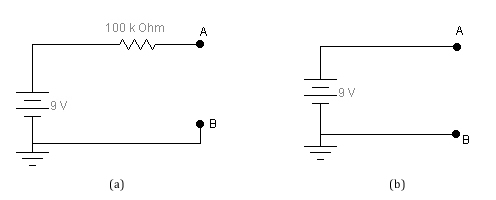
\includegraphics[width=0.66\textwidth]{images/p1-item-1.jpg}
	\caption{Estimación ideal de la caída de tensión entre los bornes A y B \\ de los circuitos (a) y (b).}
\end{figure}
\bigskip


	Adentrándonos en la parte experimental, pasaremos a medir la tensión sobre los bornes A y B de los circuitos de la \textit{Figura 2} utilizando un voltímetro analógico.
\bigskip

\begin{figure}[h]
	\centering
	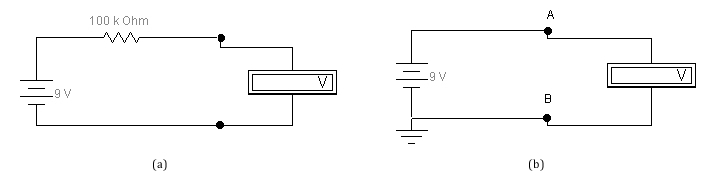
\includegraphics[width=0.94\textwidth]{images/p1-item-2.jpg}
	\caption{Estimación ideal de la caída de tensión entre los bornes A y B \\ de los circuitos (a) y (b).}
\end{figure}
\bigskip


\noindent Habiendo utilizado el voltímetro \textit{TRIPLETT 630-APLK}, se obtuvieron los siguientes resultados:
\bigskip

	\indent \textbf{Circuito (a):} $V_{medido} = 6V$ \smallskip\\
	\indent \textbf{Circuito (b):} $V_{medido} = 8,6V$ \\
	\medskip

	Al reemplazar el voltímetro analógico por uno digital (en nuestro caso se utilizó un multímetro digital \textit{UNI-T Modelo UT30F}) se obtuvieron los siguientes valores de tensión:
\bigskip

	\indent \textbf{Circuito (a):} $V_{medido} = 8,91V$ \smallskip\\
	\indent \textbf{Circuito (b):} $V_{medido} = 9,02V$ \\
	\bigskip

\newpage
\textit{¿Qué diferencia se puede observar en las mediciones?}
\medskip

	Texto texto texto texto texto texto texto texto texto texto texto texto texto texto texto texto texto texto texto texto texto texto texto texto texto texto texto texto texto texto texto texto texto texto texto texto texto texto texto texto texto texto texto texto texto texto texto texto texto texto.
\bigskip

\textit{¿A qué se atribujen esas diferencias?}
\medskip

	 Texto texto texto texto texto texto texto texto texto texto texto texto texto texto texto texto texto texto texto texto texto texto texto texto texto texto texto texto texto texto texto texto texto texto texto texto texto texto texto texto texto texto texto texto texto texto texto texto texto texto texto texto texto texto texto texto texto texto texto texto texto texto texto texto texto texto texto texto texto texto.
\bigskip

\textit{¿Como se relacionan esas diferencias con las especificaciones de los instrumentos y con los circuitos usados?}
\medskip

	Texto texto texto texto texto texto texto texto texto texto texto texto texto texto texto texto texto texto texto texto texto texto texto texto texto texto texto texto texto texto texto texto texto texto texto texto texto texto texto texto texto texto texto texto texto texto texto texto texto texto.


\bigskip
[ Colocar conclusión aquí ]



% DESARROLLO - PARTE 2
\subsection{Parte 2}



% DESARROLLO - PARTE 3
\subsection{Parte 3}


\end{document}
